%%
%% Copyright 2007, 2008, 2009 Elsevier Ltd
%%
%% This file is part of the 'Elsarticle Bundle'.
%% ---------------------------------------------
%%
%% It may be distributed under the conditions of the LaTeX Project Public
%% License, either version 1.2 of this license or (at your option) any
%% later version.  The latest version of this license is in
%%    http://www.latex-project.org/lppl.txt
%% and version 1.2 or later is part of all distributions of LaTeX
%% version 1999/12/01 or later.
%%
%% The list of all files belonging to the 'Elsarticle Bundle' is
%% given in the file `manifest.txt'.
%%

%% Template article for Elsevier's document class `elsarticle'
%% with numbered style bibliographic references
%% SP 2008/03/01
%%
%%
%%
%% $Id: elsarticle-template-num.tex 4 2009-10-24 08:22:58Z rishi $
%%
%%
\documentclass[final,1p]{elsarticle}

%% Use the option review to obtain double line spacing
%% \documentclass[preprint,review,12pt]{elsarticle}

%% Use the options 1p,twocolumn; 3p; 3p,twocolumn; 5p; or 5p,twocolumn
%% for a journal layout:
%% \documentclass[final,1p,times]{elsarticle}
%% \documentclass[final,1p,times,twocolumn]{elsarticle}
%% \documentclass[final,3p,times]{elsarticle}
%% \documentclass[final,3p,times,twocolumn]{elsarticle}
%% \documentclass[final,5p,times]{elsarticle}
%% \documentclass[final,5p,times,twocolumn]{elsarticle}

%% if you use PostScript figures in your article
%% use the graphics package for simple commands
%% \usepackage{graphics}
%% or use the graphicx package for more complicated commands
%% \usepackage{graphicx}
%% or use the epsfig package if you prefer to use the old commands
%% \usepackage{epsfig}

%% The amssymb package provides various useful mathematical symbols
\usepackage{amssymb}
\usepackage{subcaption}
%% The amsthm package provides extended theorem environments
%% \usepackage{amsthm}

%% The lineno packages adds line numbers. Start line numbering with
%% \begin{linenumbers}, end it with \end{linenumbers}. Or switch it on
%% for the whole article with \linenumbers after \end{frontmatter}.
%% \usepackage{lineno}

%% natbib.sty is loaded by default. However, natbib options can be
%% provided with \biboptions{...} command. Following options are
%% valid:

%%   round  -  round parentheses are used (default)
%%   square -  square brackets are used   [option]
%%   curly  -  curly braces are used      {option}
%%   angle  -  angle brackets are used    <option>
%%   semicolon  -  multiple citations separated by semi-colon
%%   colon  - same as semicolon, an earlier confusion
%%   comma  -  separated by comma
%%   numbers-  selects numerical citations
%%   super  -  numerical citations as superscripts
%%   sort   -  sorts multiple citations according to order in ref. list
%%   sort&compress   -  like sort, but also compresses numerical citations
%%   compress - compresses without sorting
%%
%% \biboptions{comma,round}

% \biboptions{}


\journal{GEAIO}

\begin{document}

\begin{frontmatter}

%% Title, authors and addresses

%% use the tnoteref command within \title for footnotes;
%% use the tnotetext command for the associated footnote;
%% use the fnref command within \author or \address for footnotes;
%% use the fntext command for the associated footnote;
%% use the corref command within \author for corresponding author footnotes;
%% use the cortext command for the associated footnote;
%% use the ead command for the email address,
%% and the form \ead[url] for the home page:
%%
%% \title{Title\tnoteref{label1}}
%% \tnotetext[label1]{}
%% \author{Name\corref{cor1}\fnref{label2}}
%% \ead{email address}
%% \ead[url]{home page}
%% \fntext[label2]{}
%% \cortext[cor1]{}
%% \address{Address\fnref{label3}}
%% \fntext[label3]{}

\title{Implementation of the Ground Delay Program}

%% use optional labels to link authors explicitly to addresses:
%% \author[label1,label2]{<author name>}
%% \address[label1]{<address>}
%% \address[label2]{<address>}

\author[ad1]{Ariadna Zafra}

\address[ad1]{ariadna.zafra@estudiant.upc.edu EETAC-UPC Barcelona}

%%\author[ad2]{Name2 Surname2}

%%\address[ad2]{Data contact author2}

\begin{abstract}
%% Text of abstract
The discrepancy between the available arrival slots at an airport in a given time and the demand of arrival slots can be resolve by the Ground Delay Program (GDP). In this work a GDP and a study of trends have been implemented in order to solve the capacity constraints at an airport affected, by a technical or meteorological problem with the most apropiated parameters. It has been demonstrated through simulations, the advantage of implemetation of a GDP changing the holding delay in ground delay, also a behavioral study of trends in function of radius or start time was made to justify the choice of parameters within the engagement.
\\

The simulation have been based on a typical traffic demand profile and shows the importance to select the optimum radius, which can reduce the average ground delay and the total air delay. On the other hand, a critical and realistic point of view, shows that the mathematical solution is not the real optimum due to the radius must avoid generate unnecessary delay if the conditions of the airport change, i.e exits a the tradeoff between forecasting and dynamic flexibility that minimize costs.

\end{abstract}

\begin{keyword}
GDP, ground delay, holding delay, capacity, radius, RBS, education.
%% keywords here, in the form: keyword \sep keyword
%% MSC codes here, in the form: \MSC code \sep code
%% or \MSC[2008] code \sep code (2000 is the default)

\end{keyword}

\end{frontmatter}

%%
%% Start line numbering here if you want
%%
% \linenumbers
%% main text
\section{Introduction}
\label{Sec:Sect1}

When an airport has a technical problem, meteorological bad conditions or the current congestion problems (derivate of growing air traffic demand), the Airport Acceptance Rate (AAR) decrese under the demand rate, that means that the flights arriving to airport cannot to land in their Estimate Time of Arrival (ETA). These delayted flights are doing holding delay, that generates serious problems of costs and degrade quality customer satisfaction. In order to manage the scheduled arrival flow consistent with airport's capacity, it is necessary to implement a GDP, that priorice important flights like long range or international flights over regional flights and turn the holding delay (in air) to ground delay in the original airport, removing the environmetal and economic cost implications. Section \ref{Sec:Sect2} explain the basic idea of GPD and section \ref{Sec:Sect3} resume the procedure implemented in the program, then the trends and results are explained in section \ref{Sec:Sect4} and finally the conclusion obtined in section \ref{Sec:Sect5}.


\section{GDP Idea}
\label{Sec:Sect2}

 
The Program Airport Acceptance Rate (PAAR) is defined as the AAR stimated in an airport affected by GDP, if this PAAR is lower than AAR demand induces the Delay (D). The flights affected by the GDP (i.e on the ground and inside the radio of affectation when the GDP is implemented), get a delay Figure~\ref{f:a}, changing the Estimate Time of Departure (ETD) to Controlled Time of Departure (CTD), and ETA to Controlled Time of Arrival (CTA). This is the main idea, prevent delay and wait at origin's airport, reducing expenses and informing the customers.

 \begin{figure}[h]
 \centering
 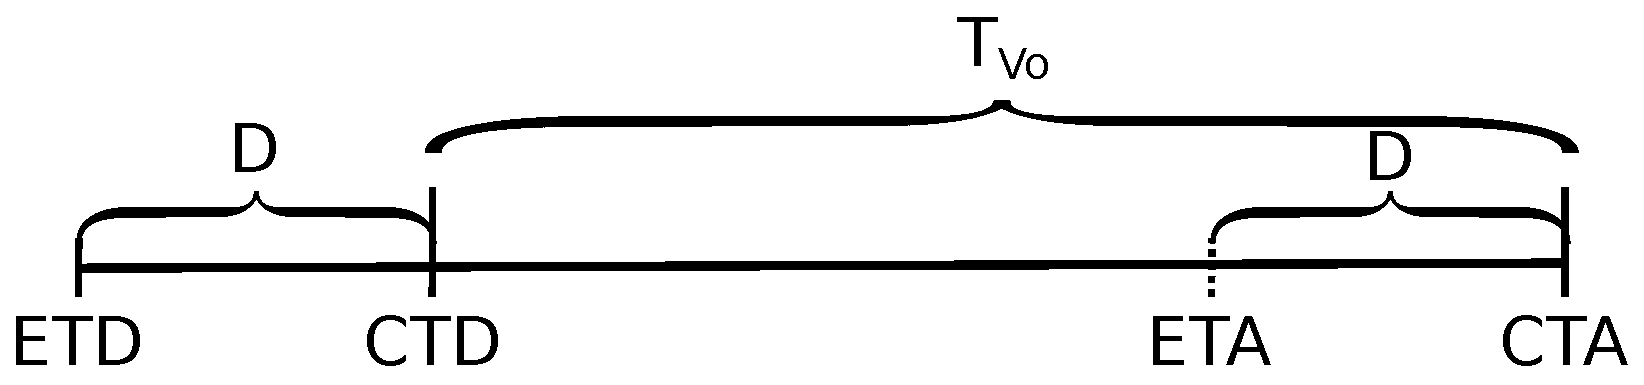
\includegraphics[width=3in]{./figs/a.eps}
 \caption{Flight Timing form Original to Destination Airport affected by GDP.}
 \label{f:a}
 \end{figure} 
 
As show in the Figure~\ref{f:agregate}, the area between blue (accumulated demand) and red \& green (accumulated capacity) delimits the total delay at GDP, in this simulation data[cita] with \textbf{total delay} of \textbf{2815 min.}

 \begin{figure}[h]
 \centering
 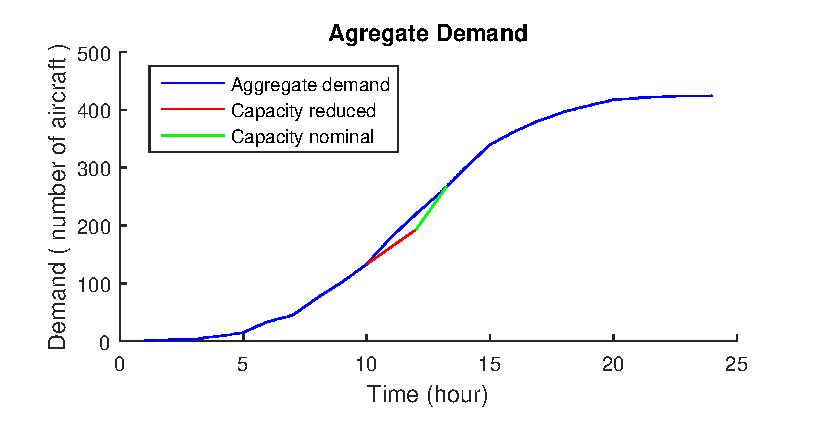
\includegraphics[width=4.5in]{./figs/agregate.eps}
 \caption{Aggregate Demand vs Aggregate Capacity.}
 \label{f:agregate}
 \end{figure} 
 
The aggregate capacity based on PAAR (red line) during the GDP between 10-12 a.m and the aggregate capacity based on AAR of 12-13:15 a.m (Figure~\ref{f:agregate}) are respectively the GDP time and the subsequent times affected by the GDP's delayed flights . When aggregate capacity and demand curves intersect at 13:15, the airport capacity already processes at nominal capacity without delay by the accumulated waiting aircraft from GDP. If a GDP is not implemented all the total delay is made by holding delay, wasting fuel and increasing ATC work.

 \begin{figure}[!hbt]
 \centering
 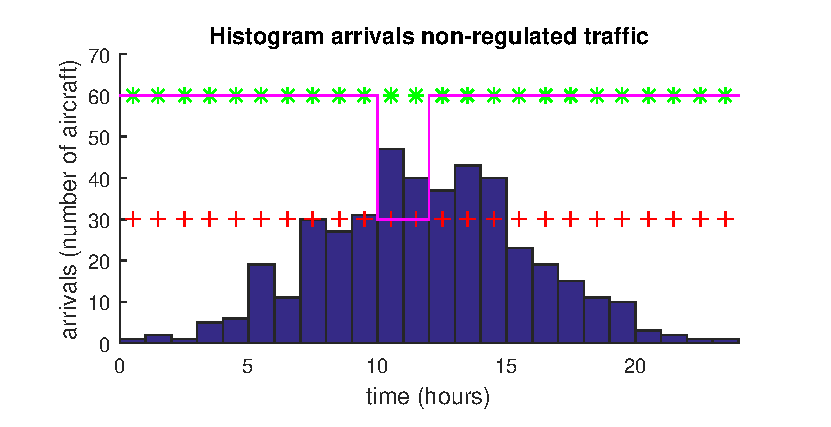
\includegraphics[width=4.5in]{./figs/agregatedemand.eps}
 \caption{Airport's Arrivals Histogram without GDP.}
 \label{f:histogram}
 \end{figure}
     
Another way to visualize is to use an arrival histogram as figure \ref{f:histogram}, the nominal ARR are the green points, the GDP PARR are the red crosses and the real capacity of the airport is the pink line. 

 \begin{figure}[h]
 \centering
 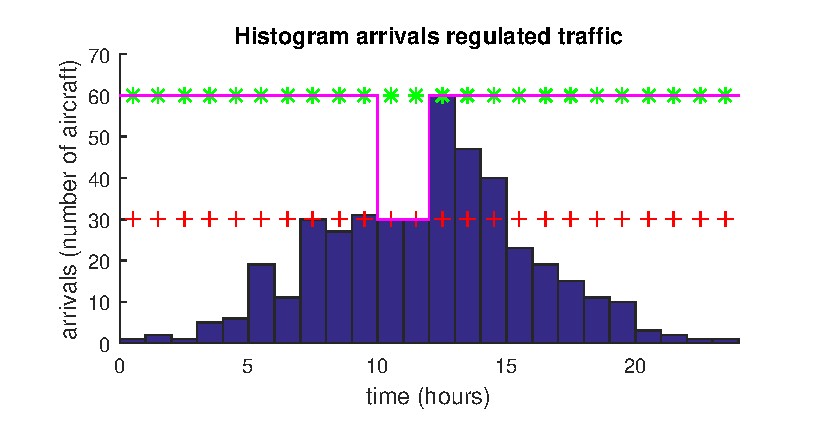
\includegraphics[width=4.5in]{./figs/GDP.eps}
 \caption{Airport's Arrivals Regulated Histogram.}
 \label{f:GDP}
 \end{figure} 
 
 All flights upper pink line between 10-12 (Figure \ref{f:histogram}) must be delayed and reassign them the free slots in the later hours until arriving at the pink line (Figure \ref{f:GDP}).

\section{GDP Simulation procedure}
\label{Sec:Sect3}

The program has been made in Matlab 2016b, with the data [cita], that can be dowload in [cita]. The main procedure of the program is a loop that redefine the basic parameter of GDP, for our case of study radius and simulate GDP using the following procedure:

\begin{enumerate}[1.]
\item Load data of flights, define GDP parameters, AAR, PAAR, start time, end time, start affected time and radius of GDP.
\item Create slots based on AAR and PAAR, compute Figure~\ref{f:agregate}, calculate total theorical delay and time when demand equals capacity .
\item Create two priority queues for all flights scheduled to arrival at the airport between GDP start and end times. Exempt flights queue contains international flights and flights departing from airport outside the GDP scope, that has precedence over the remaining and non-except flights included inside GDP. 
\item Assign slots to flights is done by queue type. Exempt flights are assigned their slots first. Then, non-exempt flights are assigned their slots based on an ordering depicted by the GDP rationing rule. For each flight, algorithm searches for the earliest slot which has the slot time equal to or later. In this work all simulations use the algorithm Ration-by-Schedule (RBS), based on the flight's original scheduled time. If there are two flights scheduled to arrive at the same time, the firts in the list get the slot, if a flight ETA is in the middle of a slot (10:01) get the next slot (10:02-10:04).
\item Compute type and value of the delay of each flight, calculate max, min, average and total delay for ground, air and sum of both.
\end{enumerate}

Finally when the loop end all the data are collected and plotted in the trend graph. In order to test the program a GDP with a radius of 1000 u. has been done by hand, checking the results, the case of study is available in [cita].

\subsection{• Real total Delay}
\label{subSec:procedure}

There is a discrepancy between the theoretical and the real delay, since the theoretical calculation is based on continuous functions (straight) but in reality the slots per hour are discrete. This discrepancy makes to delay a flight that leads at 10:01, i.e in 10:00-10:02 slot through 10:02-10:04 slot, generating an additional delay and therefore slightly larger than the theoretical. On the other hand this discrepancy is independent of GDP, so the total delay remains constant.

\section{Results and Trends}
\label{Sec:Sect4}

The interesting hours for a GDP are from 10-16 (figure \ref{f:histogram}), when the demand is greater than capacity. The simulation's parameters of these results are:
\begin{enumerate}[a.]
\item Flight data from GEAIO Deliverable [cita].
\item GDP Hdef at 8 a.m, star time at 10 a.m and end time 12 a.m.
\item PAAR equal to 30 slots per hour, AAR equal to 60 slots per hour.
\item The slots start defined at start time with the corresponding time-width.
\item GDP radius is defined inside the main loop from 500 u. to 2500 u.
\end{enumerate}

 \begin{figure}[h]
 \centering
 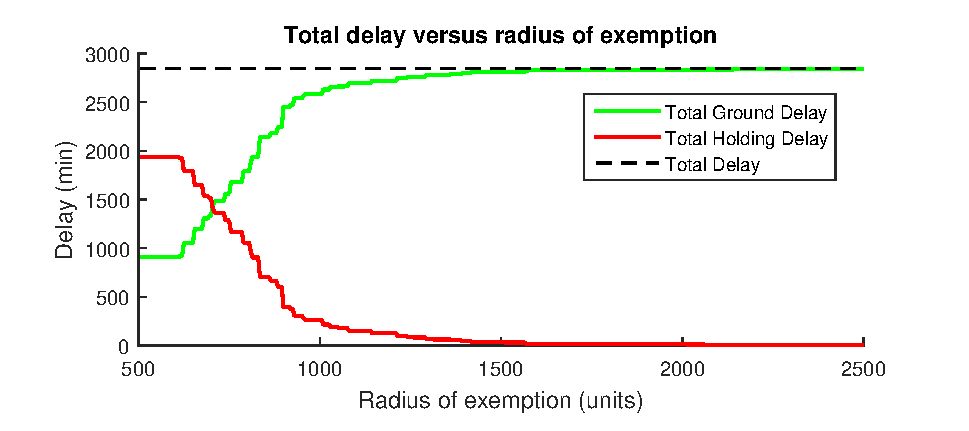
\includegraphics[width=5in]{./figs/radius.eps}
 \caption{Radius Trend of Ground, Air and Total delay.}
 \label{f:radious}
 \end{figure} 

\subsection{• GDP Theorical}
\label{subSec:theorical}

The acumulated curves and area delay are independent of radius, the results are in Figure~\ref{f:agregate}. The time when the capacity is equals to demand is at \textbf{13:15}, the GDP have a theorical \textbf{2815 min} of \textbf{total delay}, and the list of excluded or controlled aircraft, delay and type for each flight and for each radius is stored in the program memory.
The evolution of the histogram from regulated to unregulated has been recorded in Fig.~\ref{f:histogram} and Fig.~\ref{f:GDP} .

\subsection{• Hdef trends}
\label{subSec:theorical}
Hdef acts as a limiting similar to the radius, if the takeoff time is prior to Hdef the aircraft is excluded, since the time of departure is physically related to the distance, type of aircraft and the destination time, it has only iterated over the radius, assuming is static, because its trends are similar with radius results. A logical Hdef value is selected to does not interfere with the radius constraints, per example Href equal to 8 a.m.

\subsection{• Table of Results.}
\label{subSec:radius}

To get this values the radius is equal to 1000 u. and result are checked allocation each flight by hand and calculated the delay parameters, this work is publish in [cita].

\begin{table}[h]
\centering
\begin{tabular}{|l|r|r|r|}
\hline
& Delay & Holding delay & Ground delay \\
\hline
Max (min)& 106 & 13 & 106 \\
\hline
Min (min)& 0 & 0 & 2 \\
\hline
Mean (min)& 58.6818 & 2.8901 & 58.6818 \\
\hline
Total (min)& 2845 & 263 & 2582  \\
\hline
\end{tabular}
\caption{Table Values for radio of 1000 u.}
\label{tabla:table_values}
\end{table}

\subsection{• Radio trends}
\label{subSec:radius}

The real total delay need to manage the demand is 2845 min due to discrete form of slots, (discuted in section 3.1). In Figure~\ref{f:radious}, it can be seen that the larger radius more aircraft are affected by GDP, which means more holding delay change to ground delay, when the radius trend to hight values, ground delay is near to total delay (only international flight's holding delay) that is the min cost, i.e optimum radio.

 \begin{figure}[h]
 \centering
 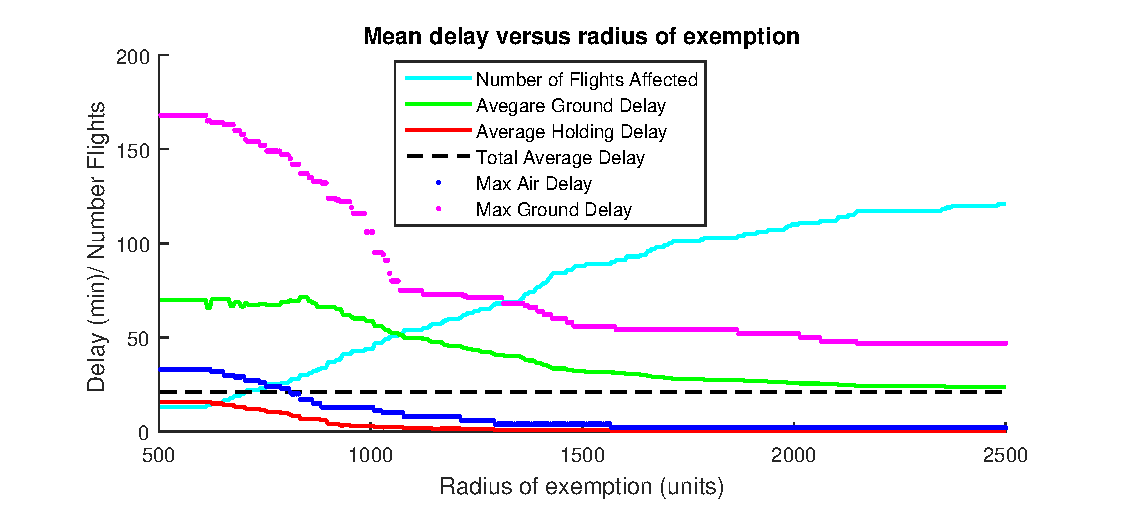
\includegraphics[width=5in]{./figs/meanradius.eps}
 \caption{Radius Trend of Average, Max and Min of Ground, Air and Total delay.}
 \label{f:meanradious}
 \end{figure} 
 
In addition, as shown in figure ~\ref{f:GDP}, if increasing the radius increases the number of flights affected, it means that the number of slot to manage is greater. If there are more slots within the GDP, it means more flexibility to reallocation, significantly reducing the maximum delay, also means that the delay is distributed among more aircraft so the average delay is reduced (related to the customer's delay and satisfaction).

\subsection{• Realistic point of view }
\label{subSec:radius}

Apparently when the radius is large enough to include all non-international aircraft it is the optimum radius. However this statement is few practical, because a large radius means to predict the capacity problem well in advance but technical problem like radar fails or runway accidents are not predictable. Also forecasting with large times means increasing the probability that the problem does not exist or disappears earlier than estimated, i.e the GDP create a not necessary delay for flight that probably are in air when the problem is fixed, therefore can not eliminate the ground delay made in origin.

\section{Conclusions}
\label{Sec:Sect5}

The case study of GDP demonstrates the advantages and the interest of implement a GDP, that minimize the impact on economic and environmental costs and increse average customer satisfaction reducing the average delay.
\\

I conclude that a GDP implement best effort of manage the reallocation of slots in order to proccess the demand of slots with the capacity, giving priority to important flights (international or long range) over regional flights, averaging the delay and reducing the maximun pic delay. Moreover allow to change air delay to ground delay avoiding waste fuel and descongesting ATC traffic near airports.
\\

Finally the study of trends of GDP based on radius, get the optimum radius when all no international flight below to GDP, that is as large as possible. The trend chart is as follows:

\begin{table}[h]
\centering
\begin{tabular}{|l|c|c|}
\hline
&Larguer Scope Radius&Shorter Scope Radius\\
\hline
Controlled Aircraft/Slots & Increases& Decreases\\
\hline
Holding Delay& Decreases& Increases\\
\hline
Ground Delay& Increases& Decreases\\
\hline
Total Delay& Constant & Constant\\
\hline
Max Delay& Decrese & Increase\\
\hline
Average Holding Delay& Decrese & Increase\\
\hline
Average Holding Delay& Decrese & Increase\\
\hline
\end{tabular}
\caption{Table Radio Trends conclusions}
\label{tabla:table_trends}
\end{table}

I concluded that the radius is to find a tradeoff between flexibility and affordable cost, that means to select a radio such that minimize the air delay, average the ground delay but do not generate too many unnecessary delays, before dynamic changes of the actual capacity compared with the estimated. For the case of study a radius around to 1200 u. is the best option because reduce around 7\% the air delay refered to the total, as can be seen in figure~\ref{f:radious} and is inside the non-exponential decrease of maxime ground delay, as can be seen in figure~\ref{f:GDP}.


\begin{thebibliography}{X}
\bibitem{Baz} \textsc{M.Ball and G.Lulli},
\textit{Ground Delay Programs:Optimizing over the Included Flight Set Based on Distance},Traffic Control Quarterly,Vol.12,2004.

\bibitem{Baz} \textsc{M.Balletal},
\textit{Total Delay Impact Study: Acomprehensive Assessment of the Cost and Impacts of Flight Delay in the United States},Tech.report,Nextor,November 2010.

\bibitem{Baz} \textsc{Gestion Aeroportuaria y del Espacio Aerio y
Investigacion Operativa ( GEAIO)},
\textit{Ground Delay Program},Atenea UPC,November 2016.

\bibitem{Baz} \textsc{Gestion Aeroportuaria y del Espacio Aerio y
Investigacion Operativa ( GEAIO)},
\textit{Data provided by the deliverable file},Atenea UPC,November 2016.

\bibitem{Baz} \textsc{A.Zafra},
\textit{Test Example made by hand},Link: November 2016.
\\
https://drive.google.com/file/d/0BwIL49dvgVJ5TDEzU2xVb1ZhSHM


\bibitem{Baz} \textsc{A.Zafra},
\textit{Matlab script code}, Github, November 2016.
\end{thebibliography}


%% The Appendices part is started with the command \appendix;
%% appendix sections are then done as normal sections
%% \appendix

%% \section{}
%% \label{}

%% References
%%
%% Following citation commands can be used in the body text:
%% Usage of \cite is as follows:
%%   \cite{key}         ==>>  [#]
%%   \cite[chap. 2]{key} ==>> [#, chap. 2]
%%

%% References with bibTeX database:

%% Authors are advised to submit their bibtex database files. They are
%% requested to list a bibtex style file in the manuscript if they do
%% not want to use elsarticle-num.bst.

%% References without bibTeX database:

% \begin{thebibliography}{00}

%% \bibitem must have the following form:
%%   \bibitem{key}...
%%

% \bibitem{}

% \end{thebibliography}

\end{document}

%%
%% End of file `elsarticle-template-num.tex'.
